\documentclass[a4paper,landscape]{article}


\usepackage{tikz}
 \usetikzlibrary{arrows}
\usetikzlibrary{fit,positioning}



\begin{document}

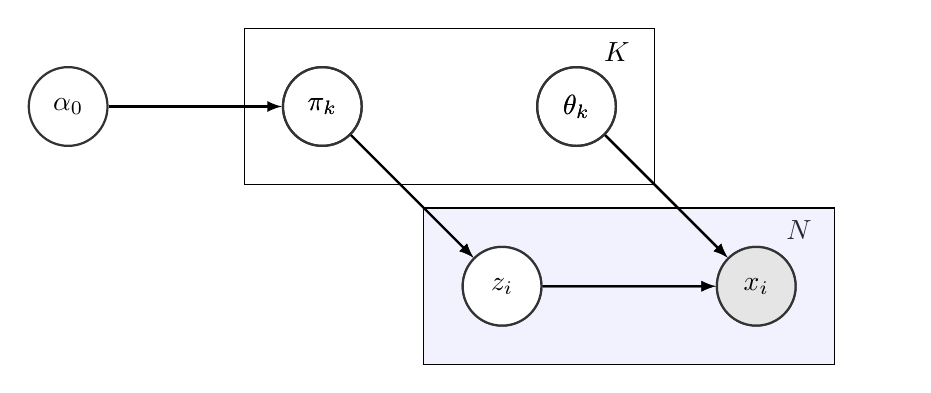
\begin{tikzpicture}[scale=.7, auto,>=latex']
\tikzstyle{main}=[circle, minimum size = 10mm, thick, draw =black!80, node distance = 22mm]
\tikzstyle{connect}=[-latex, thick]
\tikzstyle{box}=[rectangle, draw=black!100]
 \node[main] (pi) {$\pi_k$ };
 \node[main] (a) [left=of pi] {$\alpha_0$ };
 \node[main] (z_i) [below right=of pi] {$z_i$};
 \node[main, fill = black!10] (x_i) [right=of z_i] {$x_i$};
 \node[main] (theta) [above left=of x_i] {$\theta_k$};
 \path (pi) edge [connect] (z_i)
		(z_i) edge [connect] (x_i)
		(theta) edge [connect] (x_i)
		(a) edge [connect] (pi);
 \node[rectangle, inner sep=-0.5mm, fit= (z_i) (x_i),label=above right:$N$, xshift=14mm] {};
 \node[rectangle, inner sep=4.8mm,draw=black!100, fill=blue! 25, fill opacity=0.2, fit= (z_i) (x_i)] {};
 \node[rectangle, inner sep=-0.8mm, fit= (theta) (pi),label=above right:$K$, xshift=14mm] {};
 \node[rectangle, inner sep=4.8mm, draw=black! 100, fit= (theta)(pi)] {};
 \node[main] (pi) {$\pi_k$ };
 \node[main, fill = white!1] (z_i) [below right=of pi] {$z_i$};
 \node[main, fill = black!10] (x_i) [right=of z_i] {$x_i$};
 \node[main] (theta) [above left=of x_i] {$\theta_k$};
 \path (pi) edge [connect] (z_i)
		(z_i) edge [connect] (x_i)
		(theta) edge [connect] (x_i);
\end{tikzpicture}

\end{document}